\begin{frame}{Robustness result: COLORED OBJECTS}

\begin{figure}[!h]
\centering
\small
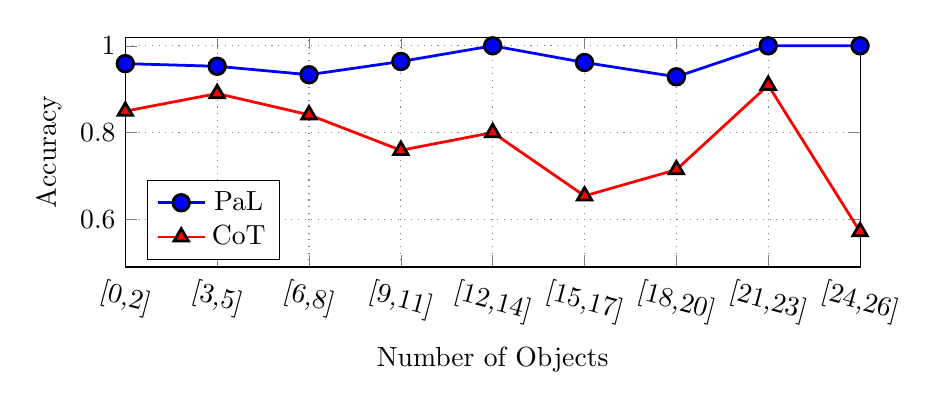
\begin{tikzpicture}
\begin{axis}[xlabel=Number of Objects,    ylabel=Accuracy, xmin=0, xmax=8, xticklabels={[0\text{,}2], [3\text{,}5], [6\text{,}8], [9\text{,}11], [12\text{,}14], [15\text{,}17],[18\text{,}20], [21\text{,}23],  [24\text{,}26]},   ymin=0.49, ymax=1.02,    xtick={0,1,2,3,4,5,6,7,8},    ytick={0.6,0.8,1.0},    legend pos=south west,    
xticklabel style = {rotate=-15},
grid = major, major grid style={dotted,gray},
width=0.9\linewidth,
height=4.5cm,
]

\addplot[    color=blue,    mark=*,  line width=1pt , mark size=3pt,
mark options={solid, fill=blue, draw=black}
]
    coordinates {
    (0,0.958904109589041) (1,0.9528145695364238) (2,0.9333333333333333) (3,0.963855421686747) (4,1.0) (5,0.9615384615384616) (6,0.9285714285714286) (7,1.0) (8,1.0)
    };
    \addlegendentry{PaL}
    
\addplot[    color=red,    mark=triangle*,  line width=1pt , mark size=3pt,
    mark options={solid, fill=red, draw=black}
]
    coordinates {
    (0,0.8493150684931506) (1,0.8899006622516556) (2,0.8408602150537634) (3,0.7590361445783133) (4,0.8) (5,0.6538461538461539) (6,0.7142857142857143) (7,0.9090909090909091) (8,0.5714285714285714)
    };
    \addlegendentry{CoT}
\end{axis}
\end{tikzpicture}
\caption{The solve rate on \textbf{Colored Objects} with respect to the number of objects included in the test question. }\label{fig:count_breakdown}
\end{figure}





\end{frame}


